\documentclass[11pt]{article}

\usepackage{pgfplots}
\usepgfplotslibrary{groupplots}
%\pgfplotsset{compat=1.14}

\usepackage{xcolor}

\definecolor{riptide}{RGB}{141,211,199}
\definecolor{pale_prim}{RGB}{255,255,179}
\definecolor{lavender_gray}{RGB}{190,186,218}
\definecolor{salmon}{RGB}{242,131,107}
\definecolor{seagull}{RGB}{128,177,211}
\definecolor{rajah}{RGB}{253,180,98}
\definecolor{yellow_green}{RGB}{198,222,119}
\definecolor{classic_rose}{RGB}{252,205,229}
\definecolor{feijoa}{RGB}{178,223,138}

\definecolor{cruise}{RGB}{179,226,205}
\definecolor{apricot}{RGB}{253,205,172}
\definecolor{periwinkle}{RGB}{203,213,232}
\definecolor{snow_flurry}{RGB}{230,245,201}
\definecolor{buttermilk}{RGB}{255,242,174}

\definecolor{sundown}{RGB}{249, 180, 181}
\definecolor{spindle}{RGB}{179,205,227}
\definecolor{tea_green}{RGB}{204,235,197}
\definecolor{languid_lavender}{RGB}{222,203,228}
\definecolor{champagne}{RGB}{254,217,166}
\definecolor{cream}{RGB}{255,255,204}


\definecolor{nonte_carlo}{RGB}{135,204,194}
\definecolor{melon}{RGB}{254,191,181}
\definecolor{granny_smith_apple}{RGB}{150,214,150}
\definecolor{mona_lisa}{RGB}{246,152,134}
\definecolor{watusi}{RGB}{254,221,207}
\definecolor{see_green}{RGB}{161,228,195}

\definecolor{moss_green}{RGB}{170,216,176}
\definecolor{opal}{RGB}{164,207,190}

\definecolor{pale_turquoise}{RGB}{172,240,242}
\definecolor{Madang}{RGB}{190,235,159}
\definecolor{pixie_green}{RGB}{183,214,170}
\definecolor{coral_andy}{RGB}{243,204,205}
\definecolor{manhattan}{RGB}{226,180,125}
\definecolor{quartz}{RGB}{219,223,238}
\definecolor{spring_sun}{RGB}{242,243,195}
\definecolor{dairy_cream}{RGB}{254,226,189}
\definecolor{surf_crest}{RGB}{205,230,208}
\definecolor{french_pass}{RGB}{195,232,246}
\definecolor{cosmos}{RGB}{248,209,210}
\definecolor{portafino}{RGB}{245,237,160}
\definecolor{sail}{RGB}{163,205,235}
\definecolor{hint_green}{RGB}{226,246,209}


\definecolor{jet_stream}{RGB}{188, 214, 210}


\definecolor{azalea}{RGB}{251, 196, 196}
\definecolor{wewak}{RGB}{244, 143, 150}
\definecolor{bittersweet}{RGB}{255,111,105}
\definecolor{sunset_orange}{RGB}{242,89,75}
\definecolor{light_coral}{RGB}{244, 127, 123}
\definecolor{carnation}{RGB}{245, 80, 86}
\definecolor{flamingo}{RGB}{237, 88, 85}
\definecolor{carmine_pink}{RGB}{231, 76, 60}
\definecolor{deep_carmine_pink}{RGB}{236, 50, 67}
\definecolor{fire_engine_red}{RGB}{210,44,41}
\definecolor{amaranth}{RGB}{234,46,73}
\definecolor{ku_crimson}{RGB}{243, 0, 25}
\definecolor{fire_engine_red}{RGB}{206, 37, 51}
\definecolor{copper_rust}{RGB}{155, 64, 74}

\definecolor{chilean_fire}{RGB}{215, 87, 44}

\definecolor{japanese_laurel}{RGB}{53, 116, 40}


\definecolor{turmeric}{RGB}{211, 178, 76}
\definecolor{saffron}{RGB}{249,193,62}
\definecolor{my_sin}{RGB}{255, 176, 59}
\definecolor{tree_poppy}{RGB}{246, 154, 27}
\definecolor{jaffa}{RGB}{240, 131, 58}
\definecolor{crusta}{RGB}{254, 127, 44}
\definecolor{tahiti_gold}{RGB}{223, 102, 36}
\definecolor{outrageous_orange}{RGB}{255, 100, 45}
\definecolor{safety_orange}{RGB}{254, 106, 0}



\definecolor{turquoise}{RGB}{41,217,194}
\definecolor{puerto_rico}{RGB}{94, 194, 166}
\definecolor{mountain_meadow}{RGB}{0, 163, 136}
\definecolor{free_speech_aquamarine}{RGB}{0, 156, 114}
\definecolor{java}{RGB}{2,190,196}


% person:
\definecolor{matisse}{RGB}{25, 104, 167}
\definecolor{shakespeare}{RGB}{85, 154, 193}
\definecolor{mona_lisa}{RGB}{246,152,134}

% gray:
\definecolor{bgc}{RGB}{245,245,245}
\definecolor{tuatara}{RGB}{67, 67, 67}
\definecolor{aluminum}{RGB}{153,153,153}
\definecolor{silver}{RGB}{191,191,191}
\definecolor{platinum}{RGB}{228,228,228}
\definecolor{mercury}{RGB}{230,230,230}
\definecolor{gallery}{RGB}{240,240,240}
\definecolor{athens_gray}{RGB}{236, 240, 241}

% nature color
\definecolor{early_dawn}{RGB}{252,243,218}
\definecolor{egg_shell}{RGB}{238, 234, 215}
\definecolor{midnight}{RGB}{0, 29, 50}
\definecolor{sundown}{RGB}{249, 180, 181}
\definecolor{sun_shade}{RGB}{255, 144, 68}
\definecolor{sushi}{RGB}{117, 168, 47}
\definecolor{tomato}{RGB}{255, 97, 56}
\definecolor{ice_cold}{RGB}{169,232,220}


% blue:
\definecolor{jelly_bean}{RGB}{45, 126, 150}
\definecolor{shakespeare}{RGB}{85, 154, 193}
\definecolor{celestial_blue}{RGB}{52, 152, 219}
\definecolor{curious_blue}{RGB}{41, 128, 185}
\definecolor{french_blue}{RGB}{0, 112, 182}
\definecolor{matisse}{RGB}{25, 104, 167}

\definecolor{biscay}{RGB}{44, 62, 80}

% green:
\definecolor{cosmic_latte}{RGB}{222, 247, 229}
\definecolor{chinook}{RGB}{163, 232, 178}
\definecolor{padua}{RGB}{121, 189, 143}
\definecolor{ocean_green}{RGB}{79, 176, 112}
\definecolor{pastel_green}{RGB}{107, 227, 135}
\definecolor{chateau_green}{RGB}{69, 191, 85}
\definecolor{RoyalBlue}{RGB}{69, 191, 85}
\definecolor{pigment_green}{RGB}{0, 175, 79}
\definecolor{fern}{RGB}{101,197,117}
\definecolor{killarney}{RGB}{56, 113, 66}
\definecolor{viridian}{RGB}{70, 137, 102}


\definecolor{jet_stream}{rgb}{0.69,0.61,0.85}
\definecolor{jelly_bean}{rgb}{0.47,0.32,0.66}




\begin{document}


\begin{figure}
\pgfplotsset{
axis background/.style={fill=gallery},
grid=both,
  xtick pos=left,
  ytick pos=left,
  tick style={
    major grid style={style=white,line width=.5pt},
    minor grid style={style=bgc, line width=.1pt},
    draw=none
    },
  ytick={200, 400},
  every x tick label/.append style={font=\tiny, yshift=2pt},
  every y tick label/.append style={rotate=90, font=\fontsize{1pt}{1pt}\selectfont, yshift=-2pt},
  ymajorgrids,
	major grid style={draw=white},
	y axis line style={opacity=0},
	tickwidth=0pt,
  title style={yshift=-5ex, font=\small},
  y label style={yshift=-5pt},
  minor tick num=1,
  height=0.4\linewidth,
  width=0.9\linewidth,
  ymin=0, ymax=600
}
\centering

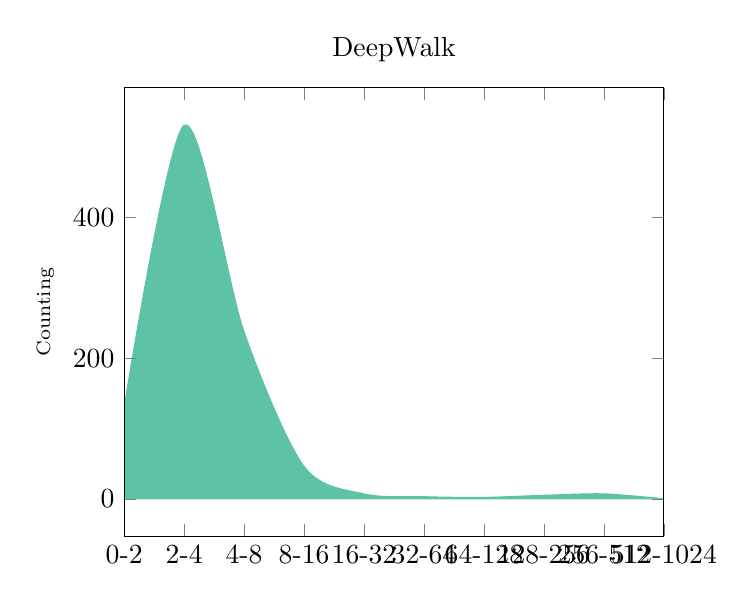
\begin{tikzpicture}
	\begin{axis}[
		smooth,
		%stack plots=y,
		area style,
		enlarge x limits=false,
		xticklabels={0-2, 2-4, 4-8, 8-16, 16-32, 32-64, 64-128, 128-256, 256-512, 512-1024},
	    xtick={1,2,3,4,5,6,7,8,9,10},
	    ylabel={\scriptsize Counting},
	    title={DeepWalk},
	    ]
	\addplot[color=puerto_rico, fill=puerto_rico] coordinates
		{(1, 130) (2, 531) (3, 237) (4, 46) (5, 7) (6, 3) (7, 2) (8, 5) (9, 7) (10, 0)}
		\closedcycle;
	\end{axis}
\end{tikzpicture}

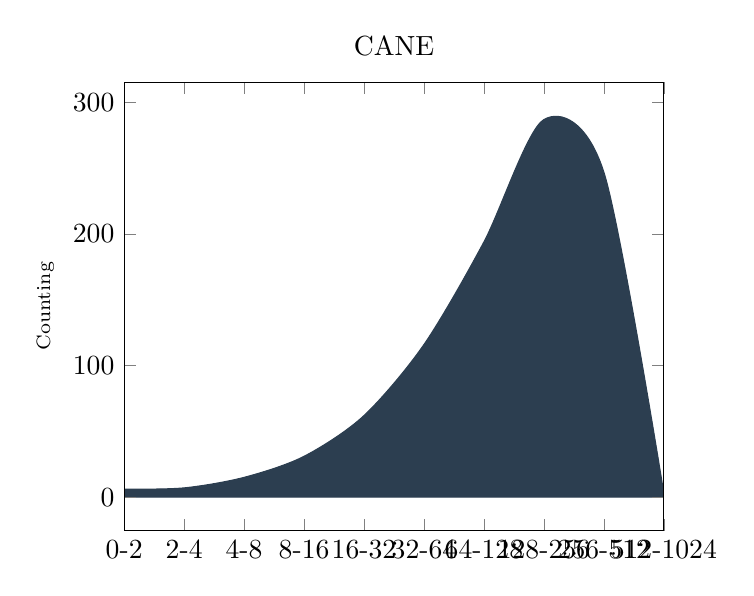
\begin{tikzpicture}
	\begin{axis}[
		smooth,
		%stack plots=y,
		area style,
		enlarge x limits=false,
		xticklabels={0-2, 2-4, 4-8, 8-16, 16-32, 32-64, 64-128, 128-256, 256-512, 512-1024},
	    xtick={1,2,3,4,5,6,7,8,9,10},
	    ylabel={\scriptsize Counting},
	    title={CANE},
	    ]
	\addplot[color=biscay, fill=biscay] coordinates
		{(1, 6) (2, 7) (3, 15) (4, 31) (5, 62) (6, 116) (7, 194) (8, 287) (9, 247) (10, 3)}
		\closedcycle;
	\end{axis}
\end{tikzpicture}

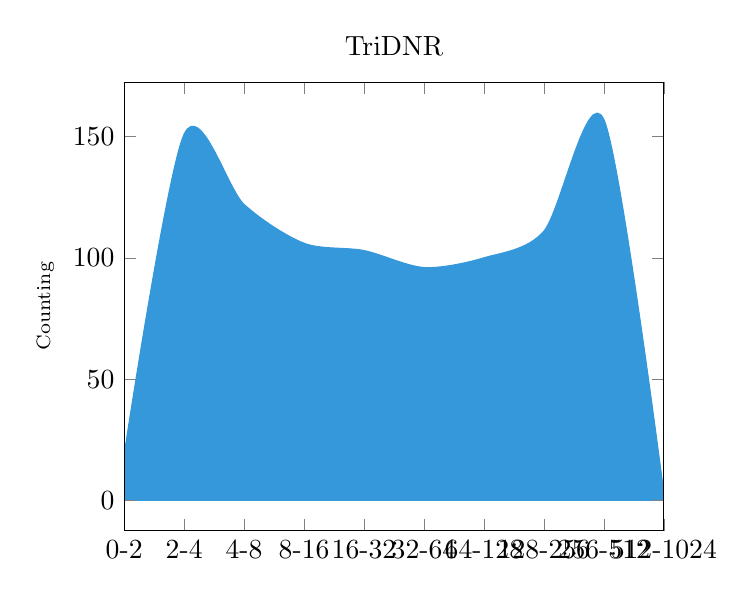
\begin{tikzpicture}
	\begin{axis}[
		smooth,
		%stack plots=y,
		area style,
		enlarge x limits=false,
		xticklabels={0-2, 2-4, 4-8, 8-16, 16-32, 32-64, 64-128, 128-256, 256-512, 512-1024},
	    xtick={1,2,3,4,5,6,7,8,9,10},
	    ylabel={\scriptsize Counting},
	    title={TriDNR},
	    ]
	\addplot[color=celestial_blue, fill=celestial_blue] coordinates
		{(1, 19) (2, 151) (3, 122) (4, 106) (5, 103) (6, 96) (7, 100) (8, 111) (9, 157) (10, 3)}
		\closedcycle;
	\end{axis}
\end{tikzpicture}

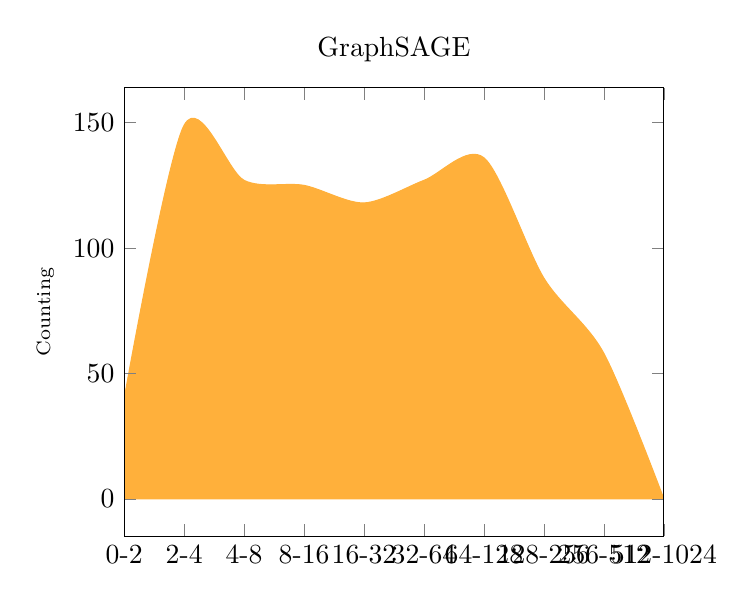
\begin{tikzpicture}
	\begin{axis}[
		smooth,
		%stack plots=y,
		area style,
		enlarge x limits=false,
		xticklabels={0-2, 2-4, 4-8, 8-16, 16-32, 32-64, 64-128, 128-256, 256-512, 512-1024},
	    xtick={1,2,3,4,5,6,7,8,9,10},
	    ylabel={\scriptsize Counting},
	    title={GraphSAGE},
	    ]
	\addplot[color=my_sin, fill=my_sin] coordinates
		{(1, 40) (2, 149) (3, 127) (4, 125) (5, 118) (6, 127) (7, 136) (8, 88) (9, 58) (10, 0)}
		\closedcycle;
	\end{axis}
\end{tikzpicture}

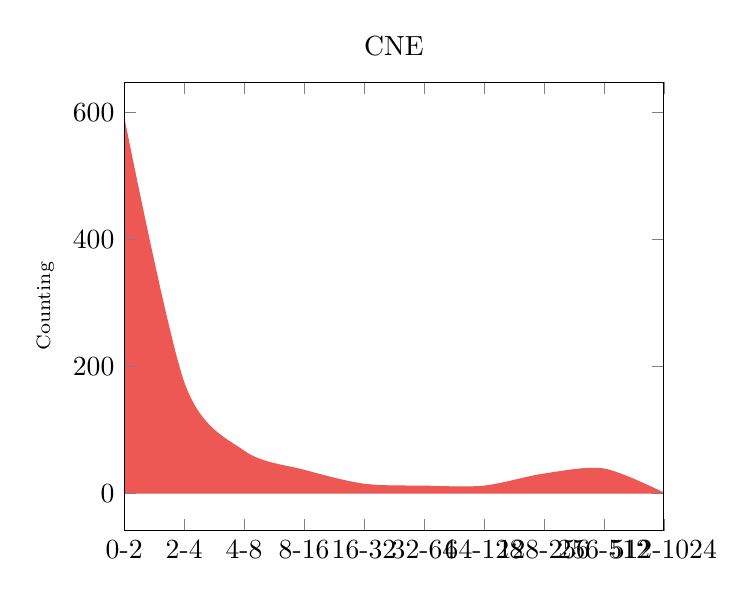
\begin{tikzpicture}
	\begin{axis}[
		smooth,
		%stack plots=y,
		area style,
		enlarge x limits=false,
		xticklabels={0-2, 2-4, 4-8, 8-16, 16-32, 32-64, 64-128, 128-256, 256-512, 512-1024},
	    xtick={1,2,3,4,5,6,7,8,9,10},
	    ylabel={\scriptsize Counting},
	    title={CNE},
	    ]
	\addplot[color=flamingo, fill=flamingo] coordinates
		{(1,589) (2,173) (3,66) (4,36) (5,14) (6,11) (7,11) (8,30) (9,38) (10,0)}
		\closedcycle;
	\end{axis}
\end{tikzpicture}

  \caption{Dist plot.}
  \label{rank_distribution}
\end{figure}



\end{document}
